
\section{Laser stand for the MAPMT characterization}
The large number of the channels in the RICH detector  poses a challenging problem for the MAPMT testing and calibration.
The RICH consists of 391 MAPMTs, resulting in a total of 25024 channels. In order to test them efficiently within a reasonable timeframe, the fully automated test stand was built to evaluate 6 MAPMTs at once, as shown in Fig.~\ref{fig:MAPMTtest}.

\begin{figure}[hbt]
	\centering
	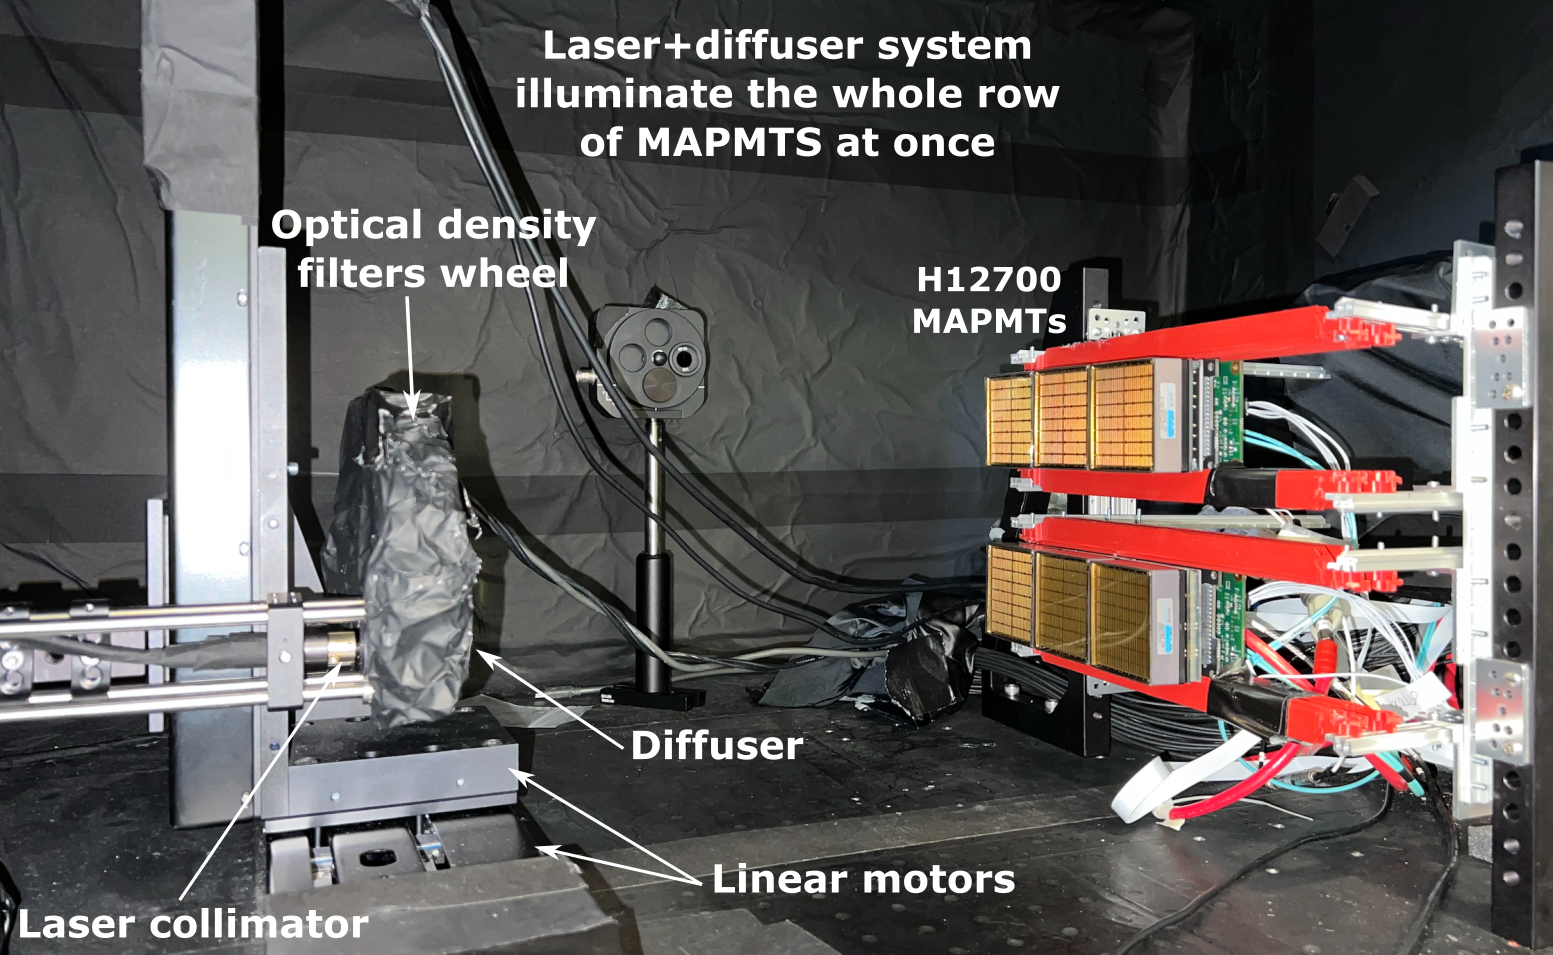
\includegraphics[width=0.95\linewidth]{figures/LaserSetup.png}
	\caption{Inner view of the laser test stand.}
	\label{fig:MAPMTtest}
\end{figure}

The test stand consists of a picosecond diode  laser PiL047X with a 470 nm wavelength, 2 long travel motorized stands to drive the laser fiber in two dimensional space for individual pixel illumination, a motorized wheel with a neutral density filter system, and 2 adapter boards for the MAPMTs with JLab designed front-end electronics boards \cite{Contalbrigo:2020}.
The laser light is directed through the fiber and attenuated to the single photon level using neutral density filters to mimic the conditions of the RICH detector.
The remotely operated filter wheel has 6 positions allowing to switch the light attenuation and evaluate MAPMT at different light intensities.
The motors can be controlled to move the focused laser beam across (see Fig.~\ref{fig:beamopt1}) the entire surface of the MAPMT entrance window and illuminate one by one all 64 pixels individually.
Alternatively, the Engineered Diffuser can be used to scatter the laser beam and produce a square pattern with a non-Gaussian intensity distribution (see Fig.~\ref{fig:beamopt2}). 
The second option is used in production mode to illuminate the full row of 3 MAPMTs at once.

All laser stand equipment is placed in a black box with non-reflective black material on the optical table. The laser interlock safety box automatically switches off the laser, as well as the front-end electronics low voltage and MAPMT high voltage, to prevent possible photomultiplier damage or human exposure to the laser light in case the front door of the black box is opened during measurements.

\begin{figure}[bt]
	\centering
	\begin{subfigure}[b]{0.628\linewidth}
		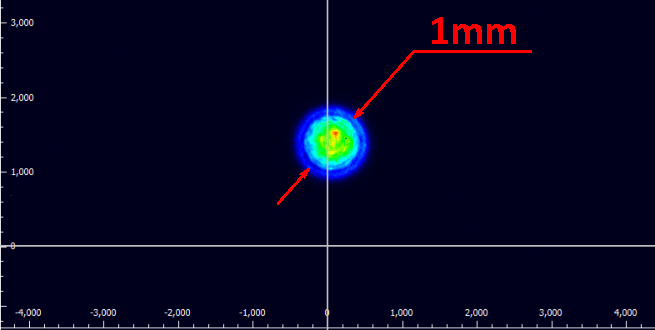
\includegraphics[width=\linewidth]{figures/beamspot.pdf}
		\caption{Focused laser beam with the dimension much less than the  MAPMT pixel size.}
		\label{fig:beamopt1}
	\end{subfigure}
	\begin{subfigure}[b]{0.354\linewidth}
		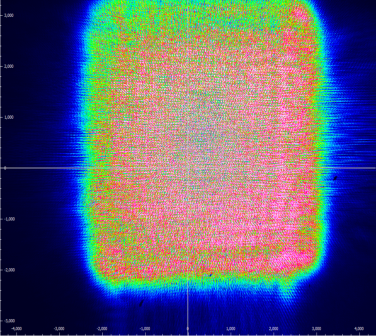
\includegraphics[width=\linewidth]{figures/beamsquare.pdf}
		\caption{Square pattern illuminating the full MAPMT surface.}
		\label{fig:beamopt2}
	\end{subfigure}
	\caption{The laser light output options.}
\end{figure}

This configuration minimizes the routine workload and allows for the evaluation of 6 MAPMTs (equivalent to 384 conventional PMTs!) at different high voltages and different light intensities within 6 hours with less than 15 minutes of human interaction used to load the MAPMTs to the front-end boards.

